%! TeX program = lualatex
\documentclass[a4paper,11pt]{report}
% packages
\usepackage{censor}
\StopCensoring
\usepackage{fontspec}
\setmainfont{EB Garamond}
% for tironian et fallback
% % \directlua{luaotfload.add_fallback
% % ("emojifallback",
% %      {"Noto Serif:mode=harf"}
% % )}
% % \setmainfont{EB Garamond}[RawFeature={fallback=emojifallback}]

\setmonofont[Scale=MatchLowercase]{Deja Vu Sans Mono}
\usepackage[a4paper,left=2cm,right=2cm,top=\dimexpr15mm+1.5\baselineskip,bottom=2cm]{geometry}
\setlength{\parindent}{0pt}

\usepackage{fancyhdr}       % Headers and footers 
\fancyhead[R]{\normalfont \leftmark}
\fancyhead[L]{}
\pagestyle{fancy}

\usepackage{microtype}      % Slightly tweak font spacing for aesthetics
\usepackage[english]{babel} % Language hyphenation and typographical rules
\usepackage{xcolor}
\definecolor{linkblue}{RGB}{0, 64, 128}
\usepackage[final, hidelinks, colorlinks = false, urlcolor = linkblue]{hyperref} 
% \newcommand{\secref}[1]{\textbf{§~\nameref{#1}}}
\newcommand{\secref}[1]{\textbf{§\ref{#1}~\nameref{#1}}}

\usepackage{changepage}     % adjust margins on the fly
\usepackage{amsmath}
\usepackage{amsmath,amssymb}

\usepackage[backend=biber, style=numeric, date=iso, urldate=iso]{biblatex}
\addbibresource{references.bib}
\DeclareFieldFormat{urldate}{Accessed #1}

\usepackage{minted}
\usemintedstyle{algol_nu}

\usepackage{pgfplots}
\pgfplotsset{width=\textwidth,compat=1.9}

\usepackage{caption}
\newenvironment{code}{\captionsetup{type=listing}}{}
\captionsetup[listing]{skip=0pt}
\setlength{\abovecaptionskip}{5pt}
\setlength{\belowcaptionskip}{5pt}

\usepackage[yyyymmdd]{datetime}
\renewcommand{\dateseparator}{--}

\usepackage{enumitem}

\usepackage{titlesec}

\author{Andrew Hayes}

\begin{document}
\begin{titlepage}
    \begin{center}

        \vfill
        % University Logo
        
\includegraphics[width=\textwidth]{./images/Logo-UGalway-2-3166136658.jpg} \\[1cm]

        % Title
        {\Huge \textbf{Iompar: Live Public Transport Tracking}} \\[0.5cm]
        
        % Department and Degree
        {\Large College of Science \& Engineering} \\[0.3cm]
        {\large Bachelor of Science (Computer Science \& Information Technology)} \\[0.5cm]

        % Report Type
        {\large \textbf{Project Report}} \\[1.5cm]

        % Author Section
        {\Large \textbf{Author:}} \\[0.2cm]
        {\large Andrew Hayes \\ 21321503 } \\[1cm]

        % Supervisor Section
        {\Large \textbf{Academic Supervisor:}} \\[0.2cm]
        {\large Dr. Adrian Clear} \\[1.5cm]

        % Date
        {\Large \today}
        \vfill
    \end{center}
\end{titlepage}

\pagenumbering{roman}
\newpage
\tableofcontents
\newpage
\setcounter{page}{1}
\pagenumbering{arabic}

% yap about mental models with regards to how filters work
% trying to make the application work the same way the user expects it to work

\chapter{Introduction}
\section{Project Overview}
\subsection{Problem Statement}
\subsection{Background}
\section{Document Structure}

\chapter{Research}
\section{Introduction}
\section{Data Sources}
\section{Similar Services}
\section{Technologies}
\subsection{Frontend Technologies}
\subsection{Backend Technologies}
\subsection{Project Management Technologies}
\section{Conclusion}

\chapter{Requirements}
\section{Functional Requirements}
\section{Non-Functional Requirements}
\section{Use Cases}
\section{Constraints}

\chapter{Backend Design \& Implementation}
\begin{figure}[H]
    \centering
    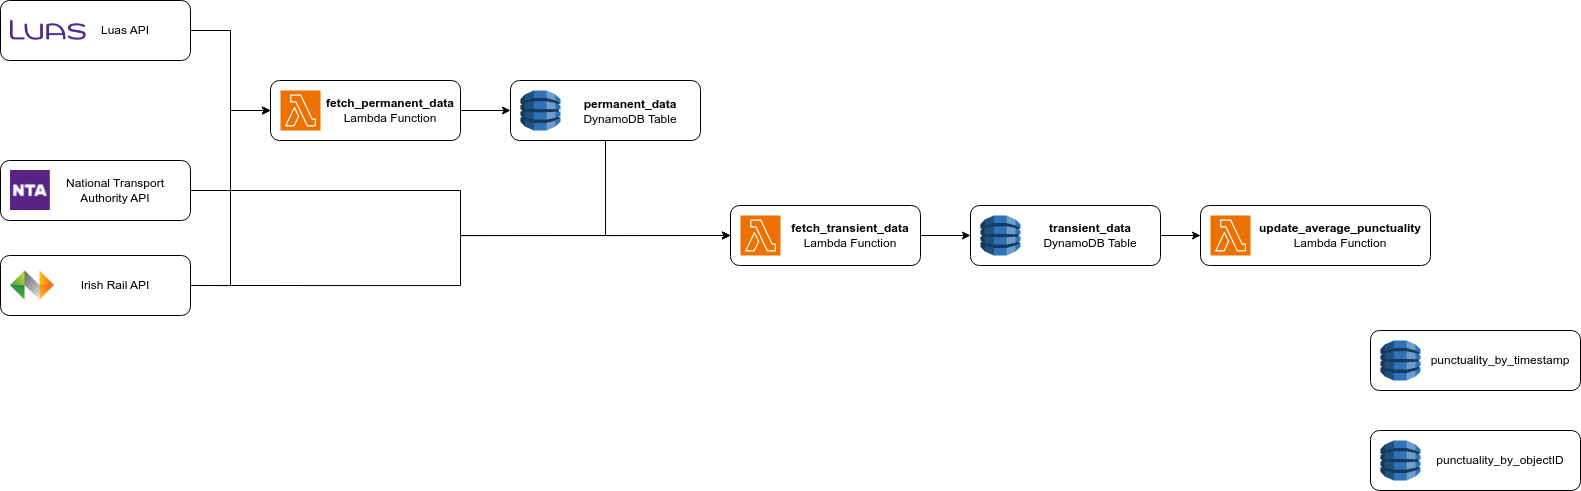
\includegraphics[width=\textwidth]{./images/diagram_all.png}
    \caption{Backend architecture}
\end{figure}

\section{Database Design}
Since the chosen database system was DynamoDB, a No-SQL database, the question of how best to separate the data is more open-ended: unlike a relational database, there is no provably correct, optimised structure of separated tables upon which to base the database design.
The decision was made that data would be separated into tables according to the type of data, how its used, and how its updated, thus allowing separation of concerns for functions which update the data and allowing different primary keys and indices to be used for different querying patterns.

\subsubsection{Permanent Data Table}
The permanent data table holds the application data which is unchanging and needs to be updated only rarely, if ever.
This includes information about bus stops, train stations, Luas stops, and bus routes.
This data does not need to be updated regularly, just on an as-needed basis.
Since this data is not temporal in nature, no timestamping of records is necessary.

\begin{code}
\begin{minted}[linenos, breaklines, frame=single]{json}
[
  {
    "objectID": "IrishRailStation-GALWY",
    "objectType": "IrishRailStation",
    "trainStationCode": "GALWY",
    "trainStationID": "170",
    "trainStationAlias": null,
    "trainStationDesc": "Galway",
    "latitude": "53.2736"
    "longitude": "-9.04696",
  },
  {
    "objectID": "BusStop-8460B5226101",
    "objectType": "BusStop",
    "busStopID": "8460B5226101",
    "busStopCode": "522611",
    "busStopName": "Eyre Square",
    "latitude": "53.2750947795551"
    "longitude": "-9.04963289544644",
  },
  {
    "objectID": "BusRoute-4520_67654",
    "objectType": "BusRoute",
    "busRouteID": "4520_67654"
    "busRouteAgencyName": "City Direct",
    "busRouteAgencyID": "7778028",
    "busRouteShortName": "411",
    "busRouteLongName": "Mount Prospect - Eyre Square",
  },
  {
    "objectType": "LuasStop",
    "objectID": "LuasStop-STS",
    "luasStopCode": "STS"
    "luasStopID": "24",
    "luasStopName": "St. Stephen's Green",
    "luasStopIrishName": "Faiche Stiabhna",
    "luasStopIsParkAndRide": "0",
    "luasStopIsCycleAndRide": "0",
    "luasStopLineID": "2",
    "luasStopZoneCountA": "1",
    "luasStopZoneCountB": "1",
    "luasStopSortOrder": "10",
    "luasStopIsEnabled": "1",
    "latitude": "53.3390722222222",
    "longitude": "-6.26133333333333",
  }
]
\end{minted}
\caption{Sample of the various types of items stored in the permanent data table}
\end{code}

Beyond what is returned for an item by its source API, two additional fields are included for each item:
the \verb|objectType| to allow for querying based on this attribute and the \verb|objectID|, an attribute constructed from an item's \verb|objectType| and the unique identifier for that item in the system from which it was sourced, thus creating a globally unique identifier for the item.
However, this attribute is \textit{not} used as the primary key for the table;
instead, it exists primarily so that each item has a unique identifier that does not need to be constructed on the fly on the frontend, thus allowing the frontend to treat specific items in specific ways.
An example of a use for this is the ``favourites'' functionality: a unique identifier must be saved for each item that is added to a user's favourites.
Defining this unique identifier in the backend rather than the frontend reduces frontend overhead (important when dealing with tens of thousands of items) and also makes the system more flexible.
While the ``favourites'' functionality is implemented fully on the frontend at present, the existence of unique identifiers for items within the table means that this functionality could be transferred to the backend without major re-structuring of the database.
\\\\
There are two ways in which a primary key can be created for a DynamoDB table\supercite{choosing-the-right-key}:
\begin{itemize}
    \item   A simple primary key, consisting solely of a \textbf{partition key}: the attribute which uniquely identifies an item, analogous to simple primary keys in relational database systems.

    \item   A composite primary key, consisting of a partition key and a \textbf{sort key}, analogous to composite primary keys in relational database systems.
            Here, the partition key determines the partition in which an item's data is stored, and the sort key is used to organise the data within that partition.
\end{itemize}

While the \verb|objectID| could be used as a partition key and thus a simple primary key, it was decided not to use the attribute for this purpose as it was not the most efficient option.
The primary function of the permanent data table is to provide data for a user when they want to display a certain type of object, such as bus stops, train stations, Luas stops, or some combination of the three.
Therefore, the most common type of query that the table will be dealing with is queries which seek to return all items of a certain \verb|objectType|.
Partitioning the table by \verb|objectID| would make querying by \verb|objectID| efficient, but all other queries inefficient, and querying by \verb|objectID| is not useful for this application.
Instead, the permanent data table uses a composite primary key, using the \verb|objectType| as the partition key and the \verb|objectID| as the sort key.
Thus, it is very efficient to query by \verb|objectType| and return, for example, all the bus stops and Luas stops in the country.
\\\\
Technically speaking, there is some redundant data in each primary by using the \verb|objectID| as the sort key when the partition key is the \verb|objectType|: since the \verb|objectID| already contains the \verb|objectType|, it is repeated.
However, the unique identifier for each item is different depending on the system from which it was sourced:
for train stations, the unique identifier is named \verb|trainStationCode|, while the unique identifier for bus stops is named \verb|busStopID|.
To use these fields as sort key, they would have to be renamed in each item to some identical title, thus adding overhead to the process of fetching data, and making the table less human-readable.
Since the \verb|objectID| was to be constructed regardless for use on the frontend, it is therefore more efficient to re-use it as the sort key, even if it does result in a few bytes of duplicated data in the primary key of each item.

% The primary key of this table is the \verb|objectID|, necessarily unique to each record in the table.
% This is constructed as a combination of the \verb|objectType| (e.g., \verb|BusStop|, \verb|IrishRailStation|) and the unique identifier for that object returned by the API from which the data was retrieved.
% The prefix of the \verb|objectType| is used here to guarantee uniqueness of the primary key in the case that two objects in the table of differing types have the same ID given to them by their respective source APIs.
% \\\\
% There are two ways in which a primary key can be created for a DynamoDB table\supercite{choosing-the-right-key}:
% \begin{itemize}
%     \item   A simple primary key, consisting solely of a \textbf{partition key}: the attribute which uniquely identifies an item, analogous to simple primary keys in relational database systems.
%
%     \item   A composite primary key, consisting of a partition key and a \textbf{sort key}, analogous to composite primary keys in relational database systems.
%             Here, the partition key determines the partition in which an item's data is stored, and the sort key is used to organise the data within that partition.
% \end{itemize}
%
% Instead of constructing a new attribute \verb|objectID| for an item, it would also be possible to avoid creating a new attribute by instead using a composite primary key, with the partition key being the item's unique identifier in the system from which it came and the sort key being the \verb|objectType|.
% This was rejected in favour of constructing a new attribute, \verb|objectID| to serve as the simple primary key for this table for a number of reasons:
% \begin{itemize}
%     \item   The uniquely identifying attribute for each item given to it by the API from which said item was sourced has a different attribute name for every API;
%             the unique identifier for bus stops is \verb|busStopID|, for train stations is \verb|trainStationCode|, et cetera.
%             To use these values as the primary key in the table, each of these attributes would have to be re-named to some single, unifying title, creating additional parsing overhead when the data is being uploaded to the table, and making the item information more difficult to read for humans.
%
%     \item   Having a single uniquely identifying attribute for each item is useful on the frontend, allowing items to be easily uniquely identified without additional processing, useful for user functionality such as adding an item to the user's ``favourites''.
%
%     \item   The query efficiency improvements typically associated with a DynamoDB composite key would not apply to the type of queries this table is designed for with such a composite key structure.
%             The data from this table will most often be queried by \verb|objectType| in this application, such as in the event that a user wants to see bus stops or train stations or both on a map.
%             The composite key would only speed up querying in the event that, for a number of different items with the same unique identifier, a query was ran on based on the type of those objects sharing an identifier, which is not a situation that is likely to arise for this application.
% \end{itemize}
%
% As mentioned in the final bullet-point above, this table is only intended for a single type of query:
% queries which seek to return all the items in the table of a certain \verb|objectType| or \verb|objectType|s, such as when a frontend user requests to see bus stops, or train stations, or Luas stops, or some combination of the three.
% Therefore, it is imperative that such queries are efficient \& fast. 
% Since we cannot partition the data 

\subsubsection{Transient Data Table}
The transient data table holds the live tracking data for each currently running public transport vehicle in the country, including information about the vehicle and its location.
Similar to the permanent data table, a unique \verb|objectID| is constructed for each item.

\begin{code}
\begin{minted}[linenos, breaklines, frame=single]{json}
[
  {
    "objectType": "IrishRailTrain",
    "latenessMessage": "On time",
    "timestamp": "1742897696",
    "trainDirection": "Southbound",
    "trainStatus": "R",
    "trainDetails": "09:41 - Maynooth to Grand Canal Dock ",
    "trainType": "S",
    "objectID": "IrishRailTrain-P656",
    "averagePunctuality": "0",
    "trainUpdate": "Departed Pelletstown next stop Broombridge",
    "trainStatusFull": "Running",
    "longitude": "-6.31388",
    "trainPublicMessage": "P656\\n09:41 - Maynooth to Grand Canal Dock (0 mins late)\\nDeparted Pelletstown next stop Broombridge",
    "trainPunctuality": "0",
    "trainPunctualityStatus": "on-time",
    "trainTypeFull": "Suburban",
    "trainDate": "25 Mar 2025",
    "latitude": "53.3752",
    "trainCode": "P656"
  },
  {
    "objectType": "Bus",
    "busScheduleRelationship": "SCHEDULED",
    "timestamp": "1742908007",
    "busID": "V598",
    "busRoute": "4538_90219",
    "busRouteAgencyName": "Bus Éireann",
    "objectID": "Bus-V598",
    "busRouteLongName": "Galway Bus Station - Derry (Magee Campus Strand Road)",
    "longitude": "-8.50166607",
    "busDirection": "1",
    "busStartDate": "20250325",
    "busRouteShortName": "64",
    "latitude": "54.2190742",
    "busTripID": "4538_114801",
    "busStartTime": "10:30:00"
  },
\end{minted}
\caption{Sample of the various types of items stored in the transient data table}
\end{code}

There are only two types of objects stored in the transient data table: Irish Rail Trains and Buses.
There is no per-vehicle data provided in the Luas API, and thus no way to track the live location of Luas trams.
For the two types of objects stored in the transient data table, additional fields are added beyond what is returned by their respective APIs (and beyond the \verb|objectType| \& \verb|objectID| fields) to augment the data.
\\\\
The following additional pieces of data are added to each \verb|IrishRailTrain| object:
\begin{itemize}
    \item   The \verb|trainStatus| \& \verb|trainType| fields are single-character codes returned by the API, representing longer strings; for example a \verb|trainStatus| of \verb|"R"| indicates that the train is \textit{running}.
            To avoid having to construct these strings on the frontend, the fields \verb|trainStatusFull| \& \verb|trainTypeFull| are automatically added to the record when the data is retrieved.

    \item   The Irish Rail API compacts much of its interesting data into a single field: \verb|trainPublicMessage|.
            This field contains the \verb|trainCode| (which is also supplied individually in its own field by the API), a string containing details about the train's origin \& terminus, a string describing how late the train is, a string containing an update about the train's current whereabouts, all separated by \verb|\\n| characters.
            This string is parsed into several additional fields to prevent additional computation on the frontend, including:
            \begin{itemize}
                \item   \verb|latenessMessage|: a human-readable string which describes whether a train is early, late, or on time.
                \item   \verb|trainDetails|: a string describing the train service itself, its start time, origin, \& terminus.
                \item   \verb|trainUpdate|: a string containing an update about the current whereabouts of the train, such as what station it last departed and what station it will visit next. 
                \item   \verb|trainPunctuality|: an integer which represents how many minutes late the train is (where a negative number indicates that the train is that many minutes early).
                \item   \verb|trainPunctualityStatus|: a whitespace-free field which gives the same information as \verb|latenessMessage| but for use in filtering rather than information presentation to the user.
                        While one of these fields could be derived from the other on the frontend, the extra computation necessary when repeated for multiple trains and multiple users dwarfs the few extra bytes in the database to store the data in the machine-readable and human-readable forms.
            \end{itemize}

    \item   The \verb|averagePunctuality| field is a field which contains the average recorded value of the \verb|trainPunctuality| for trains with that \verb|trainCode| in the database, thus giving a predictor of how early or late that particular train usually is.
\end{itemize}

The following additional pieces of data are added to each \verb|Bus| object:
\begin{itemize}
    \item   \verb|busRouteAgencyName|.
    \item   \verb|busRouteShortName|.
    \item   \verb|busRouteLongName|.
\end{itemize}

These details are not included in the response from the GTFS API, but can be obtained by looking up the given \verb|busRoute| attribute in the permanent data table to find out said information about the bus route.
In a fully-normalised relational database, this would be considered data duplication, but storing the data in both places allows for faster querying as no ``joins'' need to be performed.
\\\\
Since the primary role of the transient data table is to provide up-to-date location data about various public transport services, each item in the table is given a \verb|timestamp| attribute.
This \verb|timestamp| attribute is a UNIX timestamp in seconds which uniquely identifies the batch in which this data item was obtained.
Each train \& bus obtained in the same batch have the same \verb|timestamp|, making querying for the newest data in the table more efficient.
Because the data is timestamped, old data does not have to be deleted, saving both the overhead of deleting old data every time new data is fetched, and allowing an archive of historical data to be built up over time. 
\\\\
Since the primary type of query ran on this table will be queries which seek to return all the items of a certain \verb|objectType| (or \verb|objectType|s) for the latest timestamp, it would be ideal if the primary key could be a combination of the two for maximum efficiency in querying;
however, such a combination would fail to uniquely identify each record and thus would be inappropriate for a primary key.
Instead, the primary key must be some combination of the \verb|timestamp| attribute and the \verb|objectID| attribute.
It was decided that the partition key would be the \verb|objectID| and the sort key to be the \verb|timestamp| so that all the historical data for a given item could be retrieved efficiently.
Equivalently, the partition key could be the \verb|timestamp| and the sort key could be the \verb|objectID| which would allow for queries of all items for a given timestamp, but this was rejected on the basis that such scenarios were covered by the introduction of a Global Secondary Index.
\\\\
A \textbf{Global Secondary Index (GSI)} allows querying on non-primary key attributes by defining an additional partition and sort key from the main table\supercite{gsi}.
Unlike a primary key, there is no requirement for a GSI to uniquely identify each record in the table;
a GSI can be defined on any attributes upon which queries will be made.
The addition of GSIs to a table to facilitate faster queries is analogous to \mintinline{sql}{SELECT} queries on non-primary key columns in a relational database (and the specification of a sort key is analogous to a relational \mintinline{sql}{ORDER BY} statement);
the structured nature of a relational database means that such queries are possible by default, although an index must be created on the column in question for querying on that column to be \textit{efficient} (such as with the SQL \mintinline{sql}{CREATE INDEX} statement).
In a No-SQL database like DynamoDB, this functionality does not come for free, and instead must be manually specified.
\\\\
To facilitate efficient querying of items in the table by \verb|objectType| and \verb|timestamp|, a GSI was created with partition key \verb|objectType| and sort key \verb|timestamp|, thus making queries for the newest data on a public transport type as efficient as querying on primary key attributes.
The downside of creating a GSI is the additional storage requirements, as DynamoDB implements GSIs by duplicating the data into a separate index: efficient for querying, but less so in terms of storage usage.

\subsubsection{Average Punctuality by \texttt{objectID} Table}
To give the user punctuality predictions based off the historical data stored for a given service, it's necessary that the average punctuality be calculated.
The most obvious way to do this would be to calculate the average of the punctuality values for a given \verb|objectID| in the transient data table every time data a new data item with that \verb|objectID| is added to the transient data table.
However, this would be greatly inefficient, as it would require scanning the entire table for each item uploaded to the table, greatly slowing down the fetching of new data and consuming vast amounts of DynamoDB read/write resources.
It is also intractable, as the historical data archive in the transient table grows, it will become linearly more expensive to compute the average punctuality for an item.
\\\\
Instead, it was decided that the average punctuality for an item would be stored in a table and updated as necessary.
By storing the \verb|objectID|, the \verb|average_punctuality|, and the \verb|count| of the number of records upon which this average is based, the mean punctuality for an item can be updated on an as-needed basis in an efficient manner.
The new mean value for an item can be calculated as:
\[
  \bar{x}_{\text{new}} = \frac{\left( \bar{x}_\text{old} \times c \right) + x}{c+1}
\]
where $x$ is the punctuality value for a given item, $\bar{x}_{\text{old}}$ is the previous mean punctuality value for that item, $c$ is the count of records upon which that mean was based, and $\bar{x}_{\text{new}}$ is the new mean punctuality value.
By calculating the average punctuality in this way, the operation is $O(1)$ instead of $O(n)$, thus greatly improving efficiency. 

\begin{code}
\begin{minted}[linenos, breaklines, frame=single]{json}
[
  {
    "average_punctuality": "0.5",
    "count": "2",
    "objectType": "IrishRailTrain",
    "objectID": "IrishRailTrain-P746"
  },
  {
    "average_punctuality": "-4",
    "count": "1",
    "objectType": "IrishRailTrain",
    "objectID": "IrishRailTrain-A731"
  },
  {
    "average_punctuality": "9.333333333333333333333333333",
    "count": "3",
    "objectType": "IrishRailTrain",
    "objectID": "IrishRailTrain-E112"
  },
]
\end{minted}
\caption{Sample of items from the average punctuality by \texttt{objectID} table}
\end{code}

At the time of writing, Irish Rail is the only Irish public transport provider to offer any kind of punctuality data in their public APIs, and therefore, this table only stores items with \mintinline{json}{"objectType": "IrishRailTrain"}.
It could be argued that including this value in the table is therefore redundant, as it can be inferred, but the decision was made to include this additional value to make the table expandable and updatable.
If another transport provider were to begin to offer punctuality data via their API, this table would require no updates to start including, for example, bus punctuality data.
If the \verb|objectType| were not included, this table would have to be replaced with a re-structured table in the event that a new category of public transport items were to be added.
\\\\
In the same vein as including the \verb|objectType| in each record, the primary key for this table was created with partition key \verb|objectType| and sort key \verb|objectID|, like in the permanent data table.
This means that if an additional type of public transport were to be added to the table, querying based on that \verb|objectType| would be fast \& efficient by default.
Since the primary key of a table cannot be changed once the table has been created, not using the \verb|objectType| in the primary key would meant that adding an additional public transport type to the table would require deleting the table and starting again, or at the very least the creation of an otherwise unnecessary GSI to facilitate efficient querying.

\subsubsection{Punctuality by \texttt{timestamp} Table}
To provide historical insights such as punctuality trends over time, it is necessary to keep a record of the average punctuality for each timestamp recorded in the database.
Similarly to the punctuality by \verb|objectID| table, it is more efficient to calculate this value and store it than to calculate the average for every item in the table as the data is needed.
Unlike the punctuality by \verb|objectID| table, however, the average punctuality value for a \verb|timestamp| need never be updated, as the average is calculated for each data upload run.

\begin{code}
\begin{minted}[linenos, breaklines, frame=single]{json}
[
  {
    "average_punctuality": "0.8823529411764706",
    "timestamp": "1742908007"
  },
  {
    "average_punctuality": "1.0625",
    "timestamp": "1742905796"
  }
]
\end{minted}
\caption{Sample of items from the average punctuality by \texttt{timestamp} table}
\end{code}

The partition key for this table is the \verb|timestamp| value, and there is no need for a sort key or secondary index.

\section{API Design}
To make the data available to the frontend application, a number of API endpoints are required so that the necessary data can be requested as needed by the client.
AWS offers two main types of API functionality with Amazon API Gateway\supercite{awsapi}:
\begin{itemize}
    \item   \textbf{RESTful APIs:} for a request/response model wherein the client sends a request and the server responds, stateless with no session information stored between calls, and supporting common HTTP methods \& CRUD operations.
          AWS API Gateway supports two types of RESTful APIs\supercite{httpvsrest}:
          \begin{itemize}
              \item   \textbf{HTTP APIs:} low latency, fast, \& cost-effective APIs with support for various AWS microservices such as AWS Lambda, and native CORS support, but with limited support for usage plans and caching.
                      Despite what the name may imply, these APIs default to HTTPS and are RESTful in nature.
              \item   \textbf{REST APIs:} older \& more fully-featured, suitable for legacy or complex APIs requiring fine-grained control, such as throttling, caching, API keys, and detailed monitoring \& logging, but with higher latency, cost, and more complex set-up \& maintenance.
          \end{itemize}

    \item   \textbf{WebSocket APIs:} for real-time full-duplex communication between client \& server, using a stateful session to maintain the connection \& context.
\end{itemize}

It was decided that a HTTP API would be more suitable for this application for the low latency and cost-effectiveness.
The API functions needed for this application consist only of requests for data and data responses, so the complex feature set of AWS REST APIs is not necessary.
The primary drawback of not utilising the more complex REST APIs is that HTTP APIs do not natively support caching;
this means that every request must be processed in the backend and a data response generated, meaning potentially slower throughput over time.
However, the fact that this application relies on the newest data available to give accurate \& up-to-date location information about public transport, so the utility of caching is somewhat diminished, as the cache will expire and become out of date within minutes or even seconds of its creation.
This combined with the fact that HTTP APIs are 3.5$\times$ cheaper\supercite{apipricing} than REST APIs resulted in the decision that a HTTP API would be more suitable.
\\\\
It is important to consider the security of public-facing APIs, especially ones which accept query parameters: a malicious attacker could craft a payload to either divert the control flow of the program or simply sabotage functionality.
For this reason, no query parameter is ever evaluated as code or blindly inserted into a database query;
any interpolation of query parameters is done in such a way that they are not used in raw query strings but in parameterised expressions using the \mintinline{python}{boto3} library\supercite{boto3query}.
The AWS documentation emphasises the use of parameterised queries for database operations, in particular for SQL databases which are more vulnerable, but such attacks can be applied to any database architecture\supercite{useparameterisedqueries}. 
This, combined with unit testing of invalid API query parameters means that the risk of malicious parameter injection is greatly mitigated (although never zero), as each API endpoint simply returns an error if the parameters are invalid.

\begin{figure}[H]
    \centering
    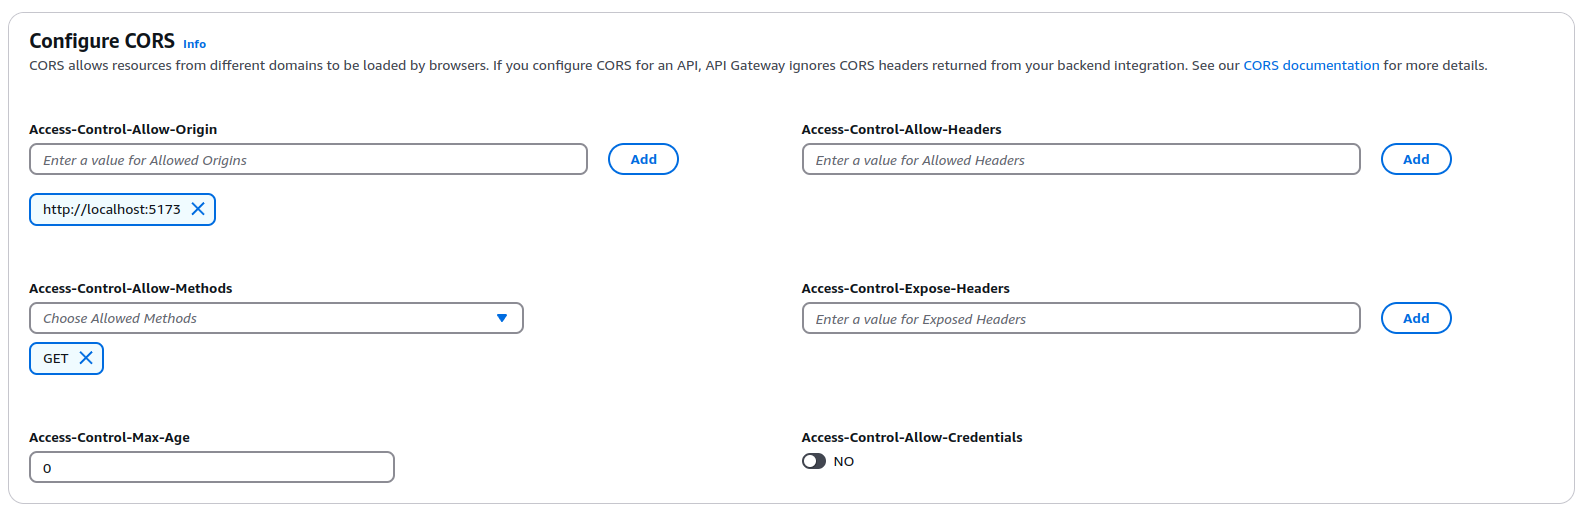
\includegraphics[width=\textwidth]{./images/api_cors_configuration.png}
    \caption{CORS configuration for the HTTP API}
\end{figure}

The Cross-Origin Resource Sharing (CORS) policy accepts only \verb|GET| requests which originate from \url{http://localhost:5173} (the URL of the locally hosted frontend application) to prevent malicious websites from making unauthorised requests on behalf of users to the API.
While the API handles no sensitive data, it is nonetheless best practice to enforce a CORS policy and a ``security-by-default'' approach so that the application does not need to be secured retroactively as its functionality expands.
If the frontend application were moved to a publicly available domain, the URL for this new domain would need to be added to the CORS policy, or else all requests would be blocked.

\subsubsection{\texttt{/return\_permanent\_data[?objectType=IrishRailStation,BusStop,LuasStop]}}
The \verb|/return_permanent_data| endpoint accepts a comma-separated list of \verb|objectType| query parameters, and returns a JSON response consisting of all items in the permanent data table which match those parameters.
If no query parameters are supplied, it defaults to returning \textit{all} items in the permanent data table.

\subsubsection{\texttt{/return\_transient\_data[?objectType=IrishRailTrain,Bus]}}
The \verb|/return_transient_data| endpoint accepts a comma-separated list of \verb|objectType| query parameters, and returns a JSON response consisting of all the items in the transient data table which match those parameters \textit{and} were uploaded to the transient data table most recently, i.e., the items which have the newest \verb|timestamp| field in the table.
Since the \verb|timestamp| pertains to the batch of data uploaded to the table in a single run, each item in the response will have the same \verb|timestamp| as all the others.
If no \verb|objectType| parameter is supplied, it defaults to returning all items from the newest upload batch. 

\subsubsection{\texttt{/return\_historical\_data[?objectType=IrishRailTrain,Bus]}}
The \verb|/return_historical_data| endpoint functions in the same manner as the \verb|/return_transient_data| endpoint, with the exception that it returns matching items for \textit{all} \verb|timestamp| values in the table, i.e., it returns all items of the given \verb|objectTypes| in the transient data table. 

\subsubsection{\texttt{/return\_luas\_data?luasStopCode=<luas\_stop\_code>}}
The \verb|/return_luas_data| returns incoming / outgoing tram data for a given Luas stop, and is just a proxy for the Luas real-time API.
Since the Luas API returns data only for a queried station and does not give information about individual vehicles, the Luas data for a given station is only fetched on the frontend when a user requests it, as there is no information to plot on the map beyond a station's location.
However, this request cannot be made from the client to the Luas API, as the Luas API's CORS policy blocks requests from unauthorised domains for security purposes;
this API endpoint acts as a proxy, accepting API requests from the \verb|localhost| domain and forwarding them to the Luas API, and subsequently forwarding the Luas API's response back to the client.
\\\\
This endpoint requires a single \verb|luasStopCode| query parameter for each query to identify the Luas stop for which incoming / outgoing tram data is being requested.

\subsubsection{\texttt{/return\_station\_data?stationCode=<station\_code>}}
The \verb|return_station_data| returns information about the trains due into a given station in the next 90 minutes.
This data is only shown to a user if requested for a specific station, so it is not stored in a DynamoDB table.
Like the \verb|/return_luas_data| endpoint, it too is just a proxy for an (Irish Rail) API, the CORS policy of which blocks requests from any unauthorised domain for security purposes.
It requires a single \verb|stationCode| query parameter for each query to identify the train station for which the incoming train data is being requested.

% \subsubsection{\texttt{/return\_punctuality\_by\_objectID[?objectID=<object\_id1>,<object\_id2>]}}
% The \verb|/return_punctuality_by_objectID| endpoint returns the contents of the \verb|punctuality_by_objectID| DynamoDB table. 
% It accepts a comma-separated list of \verb|objectID|s as query parameters, and defaults to returning the average punctuality for \textit{all} items in the table if no \verb|objectID| is specified.

\subsubsection{\texttt{/return\_punctuality\_by\_timestamp[?timestamp=<timestamp>]}}
The \verb|/return_punctuality_by_timestamp| returns the contents of the \verb|punctuality_by_timestamp| DynamoDB table.
It accepts a comma-separated list of \verb|timestamp|s, and defaults to returning the average punctuality for \textit{all} \verb|timestamp|s in the table if no \verb|timestamp| is specified. 

\subsubsection{\texttt{/return\_all\_coordinates}}
The \verb|/return_all_coordinates| endpoint returns a JSON array of all current location co-ordinates in the transient data table for use in statistical analysis.

\section{Serverless Functions}
All the backend code \& logic is implemented in a number of serverless functions, triggered as needed.

\subsubsection{\mintinline{python}{fetch_permanent_data}}
The \verb|fetch_permanent_data| Lambda function is used to populate the permanent data table.
As the data in question changes rarely if ever, this function really need only ever be triggered manually, such as when a new train station is opened or a new bus route created.
However, for the sake of completeness and to avoid the data being out of date, a schedule was created with \textbf{Amazon EventBridge} to run the function every 28 days to ensure that no changes to the data are missed.
Like all other schedules created for this application, the schedule is actually disabled at present to avoid incurring unnecessary AWS bills, but can be enabled at any time with the click of a button.

\begin{figure}[H]
    \centering
    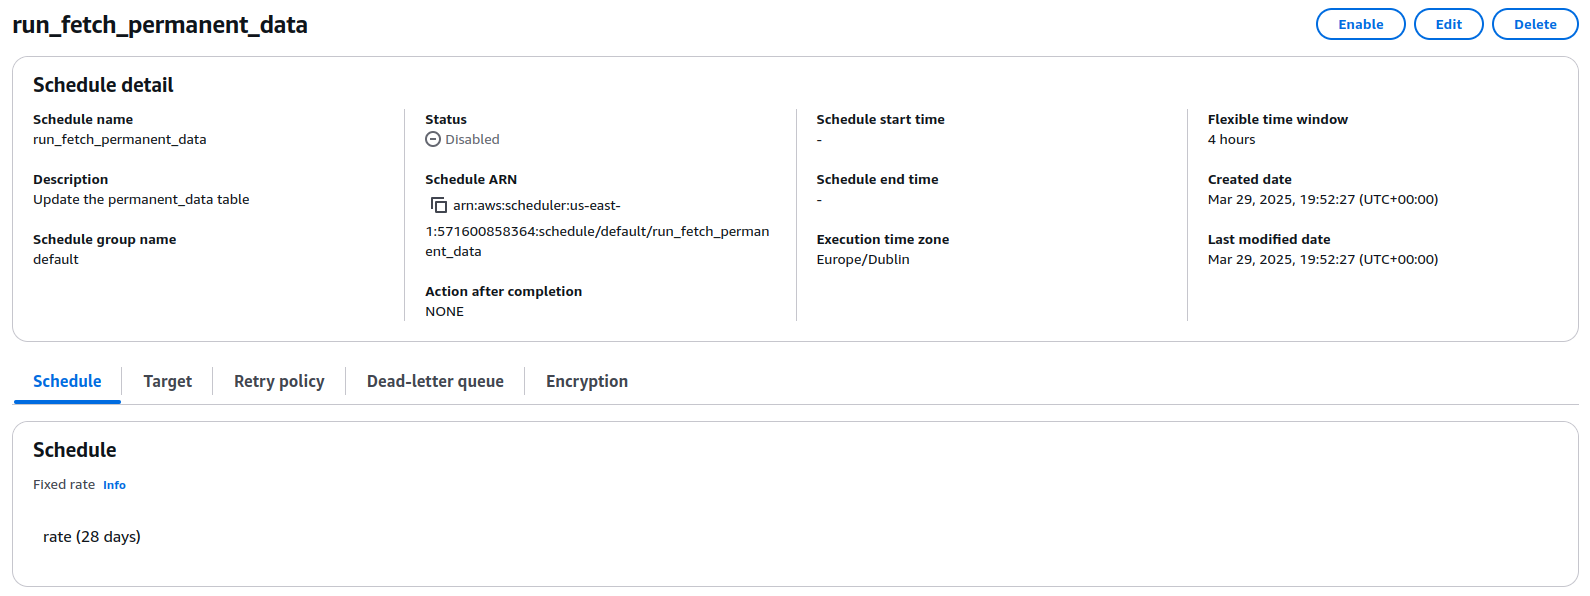
\includegraphics[width=\textwidth]{./images/fetch_permanent_data_schedule.png}
    \caption{Screenshot of the Amazon EventBridge schedule to run the \mintinline{python}{fetch_permanent_data} Lambda function}
\end{figure}

The \verb|fetch_permanent_data| function retrieves Irish Rail Station data directly from the Irish Rail API, but Luas stop data and bus data are not made available through an API;
instead, the Luas stop data is made available online in a tab-separated \verb|TXT| file, and the bus stop \& bus route data are available online in comma-separated \verb|TXT| files distributed as a single ZIP file.
This makes little difference to the data processing however, as downloading a file from a server and parsing its contents is little different in practice from downloading an API response from a server and parsing its contents.
The function runs asynchronously with a thread per type of data being fetched (train station data, Luas stop data, and bus stop \& route data), and once each thread has completed, batch uploads the data to the permanent data table, overwriting its existing contents.

\subsubsection{\mintinline{python}{fetch_transient_data}}
The \verb|fetch_transient_data| function operates much like the \verb|fetch_transient_data| function, but instead updates the contents of the transient data table.
It runs asynchronously, with a thread per API being accessed to speed up execution;
repeated requests to an API within a thread are made synchronously to avoid overloading the API.
For example, retrieving the type (e.g., Mainline, Suburban, Commuter) of the trains returned by the Irish Rail API requires three API calls:
the Irish Rail API allows the user to query for all trains or for trains of a specific type but it does not return the type of the train in the API response.
Therefore, if a query is submitted for all trains, there is no way of knowing which train is of which type.
Instead, the function queries each type of train individually, and adds the type into the parsed response data.
\\\\
Additionally, the \verb|return_punctuality_by_objectID| function is called when processing the train data so that each train's average punctuality can be added to its data for upload.
Somewhat unintuitively, it transpired that the most efficient way to request this data was to request all data from the punctuality by \verb|objectID| data table rather than individually request each necessary \verb|objectID|;
this means that much of the data returned is redundant, as many of the trains whose punctualities are returned are not running at the time and so will not be uploaded, but it means that the function is only ran once, and so only one function invocation, start-up, database connection, and database query have to be created.
It's likely that if bus punctuality data were to become available in the future, this approach would no longer be the most efficient way of doing things, and instead a \verb|return_punctuality_by_objectType| function would be the optimal solution.
\\\\
The bus data API doesn't return any information about the bus route beyond a bus route identifier, so the permanent data table is queried on each run to create a dictionary (essentially a Python hash table\supercite{pythondict}) linking bus route identifiers to information about said bus route (such as the name of the route).
As the bus data is being parsed, the relevant bus route data for each vehicle is inserted.
Once all the threads have finished executing, the data is uploaded in a batch to the transient data table, with each item timestamped to indicate which function run it was retrieved on.
\\\\
This function is ran as part of an \textbf{AWS Step Function} with a corresponding Amazon EventBridge schedule (albeit disabled at present).
A step function is an AWS service which facilitates the creation of state machines consisting of various AWS microservices to act as a single workflow.
The state machine allows multiple states and transitions to be defined, with each state representing a step in the workflow and the transitions representing how the workflow moves from one state to another and what data is transferred.
Step functions have built-in error handling and retry functionality, making them extremely fault-tolerant for critical workflows.

\begin{figure}[H]
    \centering
    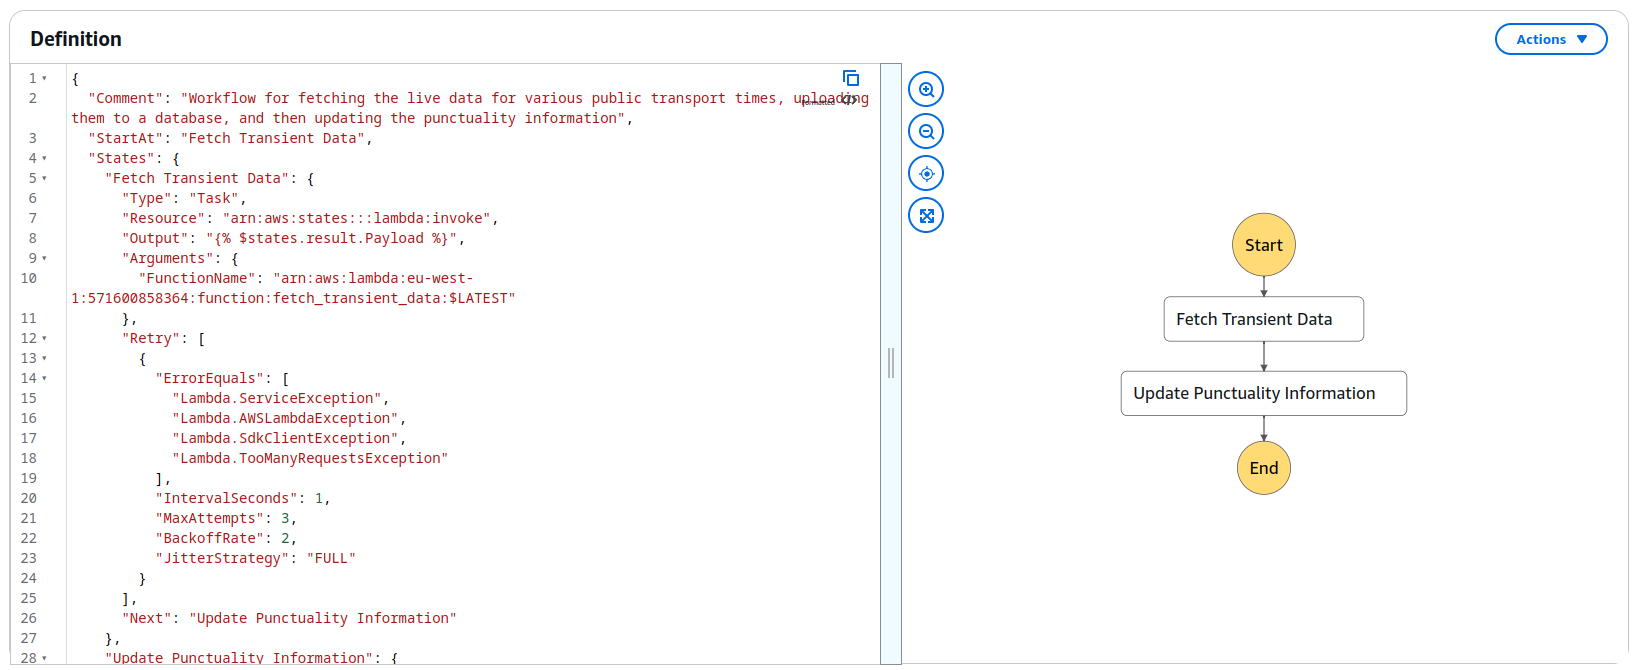
\includegraphics[width=\textwidth]{./images/get_live_data_definiton.png}
    \caption{Screenshot of the \texttt{get\_live\_data} step function definition}
\end{figure}

The step function runs the \verb|fetch_transient_data| function and then runs the \verb|update_average_punctuality| function, if and only if the \verb|fetch_transient_data| function has completed successfully.
This allows the average punctuality data to be kept up to date and in sync with the transient data, and ensures that they do not become decoupled and therefore incorrect.
This step function is triggered by a (currently disabled) Amazon EventBridge schedule which runs the function once a minute, which is the maximum frequency possible to specify within a cron schedule, and suitable for this application as the APIs from which the data is sourced don't update much more frequently than that.
Furthermore, the data from which bus data is sourced will time out if requests are made too frequently, so this value was determined to be appropriate after testing to avoid overwhelming the API or getting timed-out. 
It is possible to run EventBridge schedules even more frequently using the \textit{rate-based schedule} schedule type instead of the \textit{cron-based schedule} schedule type but a more frequent schedule would be inappropriate for this application.

\subsubsection{\mintinline{python}{update_average_punctuality}}
The \verb|update_average_punctuality| function runs after \verb|fetch_transient_data| in a step function and populates the average punctuality by \verb|objectID| and average punctuality by \verb|timestamp| tables to reflect the new data collected by \verb|fetch_transient_data|.
For each item in the new data, it updates the average punctuality in the average punctuality by \verb|objectID| table according to the aforementioned formula:
\[
  \bar{x}_{\text{new}} = \frac{\left( \bar{x}_\text{old} + c \right) + x}{c + 1}
\]

As the function iterates over each item, it adds up the total punctuality and then divides this by the total number of items processed before adding it to the average punctuality by \verb|timestamp| table, where the \verb|timestamp| in question is the \verb|timestamp| that the items were uploaded with (the \verb|timestamp| of the \verb|fetch_transient_data| run which created them).
\\\\
There are a number of concerns that one might reasonably have about using the mean punctuality for the average displayed to users:
\begin{itemize}
  \item   Means are sensitive to outliers, meaning that if, for example, a train is very late just once but very punctual the rest of the time, its average punctuality could be misleading.
  \item   The punctuality variable is an integer that can be positive or negative, which could have the result that the positive \& negative values could cancel each other out for a train that is usually either very late or very early, giving the misleading impression of an average punctuality close to zero.
  \item   Considering the entire history of a train for its average punctuality may not be reflective of recent trends:
          a train may historically have been consistently late, but become more punctual as of late and therefore the average punctuality may not be reflective of its recent average punctuality. 
\end{itemize}

These questions were carefully considered when deciding how to calculate the average punctuality, but it was decided that the mean would nonetheless be the most appropriate for various reasons:
\begin{itemize}
  \item   The mean lends itself to efficient calculation with the $O(1)$ formula described above.
          No other average can be calculated in so efficient a manner:
          the median requires the full list of punctualities to be considered to determine the new median, and the mode requires at the very least a frequency table of all the punctualities over time to determine the new mode, which requires both additional computation and another DynamoDB table.

  \item   Similarly, considering only recent data would destroy the possibility for efficient calculation:
          the mean could not be updated incrementally, and instead a subset of the historic punctualities would have to be stored and queried for each update.

  \item   The outlier sensitivity is addressed by the sheer number of items that are considered for the mean:
          since this will be updated every minute of every day, an outlier will quickly be drowned out with time.

  \item   Finally, the average is being calculated so that it can be shown to the user and so that they can make decisions based off it.
          The average person from a non-technical or non-mathematical background tends to assume that any average value is a mean value, and so it would only serve to confuse users if they were given some value that did not mean what they imagined it to mean.
          While calculating additional different measures of averages would be possible, displaying them to the user would likely be at best not useful and at worst confusing, while also greatly increasing the computation and storage costs.
          This aligns with the second of Nielsen's famous \textit{10 Usability Heuristics for User Interface Design}, which were consulted throughout the design process: ``\textbf{Match between the System and the Real World:} The design should speak the users' language. Use words, phrases, and concepts familiar to the user, rather than internal jargon''\supercite{nielsenheuristics}.
\end{itemize}

For these reasons, it was decided that the mean was the most suitable average to use.

\subsubsection{\mintinline{python}{return_permanent_data}}
The \verb|return_permanent_data| function is the Lambda function which is called when a request is made from the client to the \verb|/return_permanent_data| API endpoint.
It checks for a comma-separated list of \verb|objectType| parameters in the query parameters passed from the API event to the Lambda function, and scans the permanent data table for every item matching those \verb|objectType|s.
If none are provided, it returns every item in the table, regardless of type.
It returns this data as a JSON string.
\\\\
When this function was first being developed, the permanent data table was partitioned by \verb|objectID| alone with no sort key, meaning that querying was very inefficient.
When the table was re-structured to have a composite primary key consisting of the \verb|objectType| as the partition key and the \verb|objectID| as the sort key, the \verb|return_permanent_data| function was made 10$\times$ faster:
the average execution time was reduced from $\sim$10 seconds to $\sim$1 second, demonstrating the critical importance of choosing the right primary key for the table.

\subsubsection{\mintinline{python}{return_transient_data}}
The \verb|return_transient_data| function is the Lambda function which is called when a request is made from the client to the \verb|/return_transient_data| API endpoint.
Like \verb|return_permanent_data|, it checks for a comma-separated list of \verb|objectType| parameters in the query parameters passed from the API event to the Lambda function, and scans the permanent data table for every item matching those \verb|objectType|s.
If none are provided, it returns every item in the table, regardless of type.
\\\\
Similar to \verb|return_permanent_data|, when this function was originally being developed, there was no GSI on the transient data table to facilitate efficient queries by \verb|objectType| and \verb|timestamp|;
the addition of the GSI and updating the code to exploit the GSI resulted in an average improvement in run time of $\sim$8$\times$, thus demonstrating the utility which GSIs can provide.

\subsubsection{\mintinline{python}{return_punctuality_by_objectID}}
The \verb|return_punctuality_by_objectID| function is invoked by the \verb|fetch_transient_data| function to return the contents of the punctuality by \verb|objectID| table. 
It accepts a list of \verb|objectID|s and defaults to returning all items in the table if no parameters are provided.

\subsubsection{\mintinline{python}{return_punctuality_by_timestamp}}
The \verb|return_punctuality_by_timestamp| function is similar to \verb|return_punctuality_by_objectID| but runs when invoked by an API request to the \verb|/return_punctuality_by_timestamp| endpoint and simply returns a list of JSON objects consisting of a \verb|timestamp| and an \verb|average_punctuality|.
It is used primarily to graph the average punctuality of services over time.

\subsubsection{\mintinline{python}{return_all_coordinates}}
The \verb|return_all_coordinates| function is used to populate the co-ordinates heatmap in the frontend application which shows the geographical density of services at the present moment.
It accepts no parameters, and simply scans the transient data table for the newest items and returns their co-ordinates.

\subsubsection{\mintinline{python}{return_historical_data}}
The \verb|return_historical_data| function operates much like the \verb|return_transient_data| function, accepting a list of \verb|objectType|s or defaulting to all \verb|objectType|s if none are specified, with the only difference being that this function does not consider the \verb|timestamp|s of the data and just returns all data in the transient data table.
This function, along with its corresponding API endpoint exist primarily as a debugging \& testing interface, although they also give a convenient access point for historical data analysis should that be necessary.

\subsubsection{\mintinline{python}{return_luas_data}}
The \verb|return_luas_data| function is a simple proxy for the Luas API which accepts requests from the client and forwards them to the Luas API to circumvent the Luas API's restrictive CORS policy which blocks requests from unauthorised domains.
It simply accepts a \verb|luasStopCode| parameter, and makes a request to the Luas API with said parameter, parses the response from XML into JSON, and returns it.

\subsubsection{\mintinline{python}{return_station_data}}
Like \verb|return_luas_data|, the \verb|return_station_data| is a proxy for the Irish Rail API so that requests can be made as needed from the client's browser to get data about incoming trains due into a specific section without running afoul of Irish Rail's CORS policy.
It also accepts a single parameter (\verb|stationCode|) and makes a request to the relevant endpoint of the Irish Rail API, and returns the response (parsed from XML to JSON).


\chapter{Frontend Design \& Implementation}
The frontend design is built following the Single-Page-Application (SPA)\supercite{spa} design pattern using the React Router\supercite{reactrouter} library, meaning that the web application loads a single HTML page and dynamically updates content as the user interacts with the application, without reloading the webpage. 
Since there is just one initial page load, the content is dynamically updated via the DOM using JavaSript rather than by requesting new pages from the server;
navigation between pseudo-pages is managed entirely using client-side routing for a smoother \& faster user experience since no full-page reloads are necessary.
\\\\
The web application is split into two ``pages'':
\begin{itemize}
  \item   The home (or map) page, which is the main page that displays live location data \& service information to the user.
          This page is where the user will spend the majority of their time, and where the majority of the functionality is delivered.
  \item   The statistics page, which is used to deliver statistical insights about the data to the user.
          This page is for providing deeper insights into the stored data on a collective basis, rather than on a per-service basis.
\end{itemize}

The web application follows the Container/Presentational Pattern\supercite{containerpresentational}, which enforces separation of concerns by separating the presentational logic from the application logic.
This is done by separating the functionality into two classes of components:
\begin{itemize}
  \item   \textbf{Container Components:} those which fetch the data, process it, and pass it to the presentational components which are contained by their container components, i.e., the presentational components are children of the container components.
  \item   \textbf{Presentational Components:} those which display the data it receives from the container components to the user as it is received.
          This makes the components highly re-usable, as there isn't specific data processing handling logic within them.
\end{itemize}

React components are reusable, self-contained pieces of the UI which act as building blocks for the application\supercite{reactcomponents};
they can receive properties from their parent components, manage their own internal state, render other components within themselves, and respond to events.

\section{Main Page}
\begin{figure}[H]
    \centering
    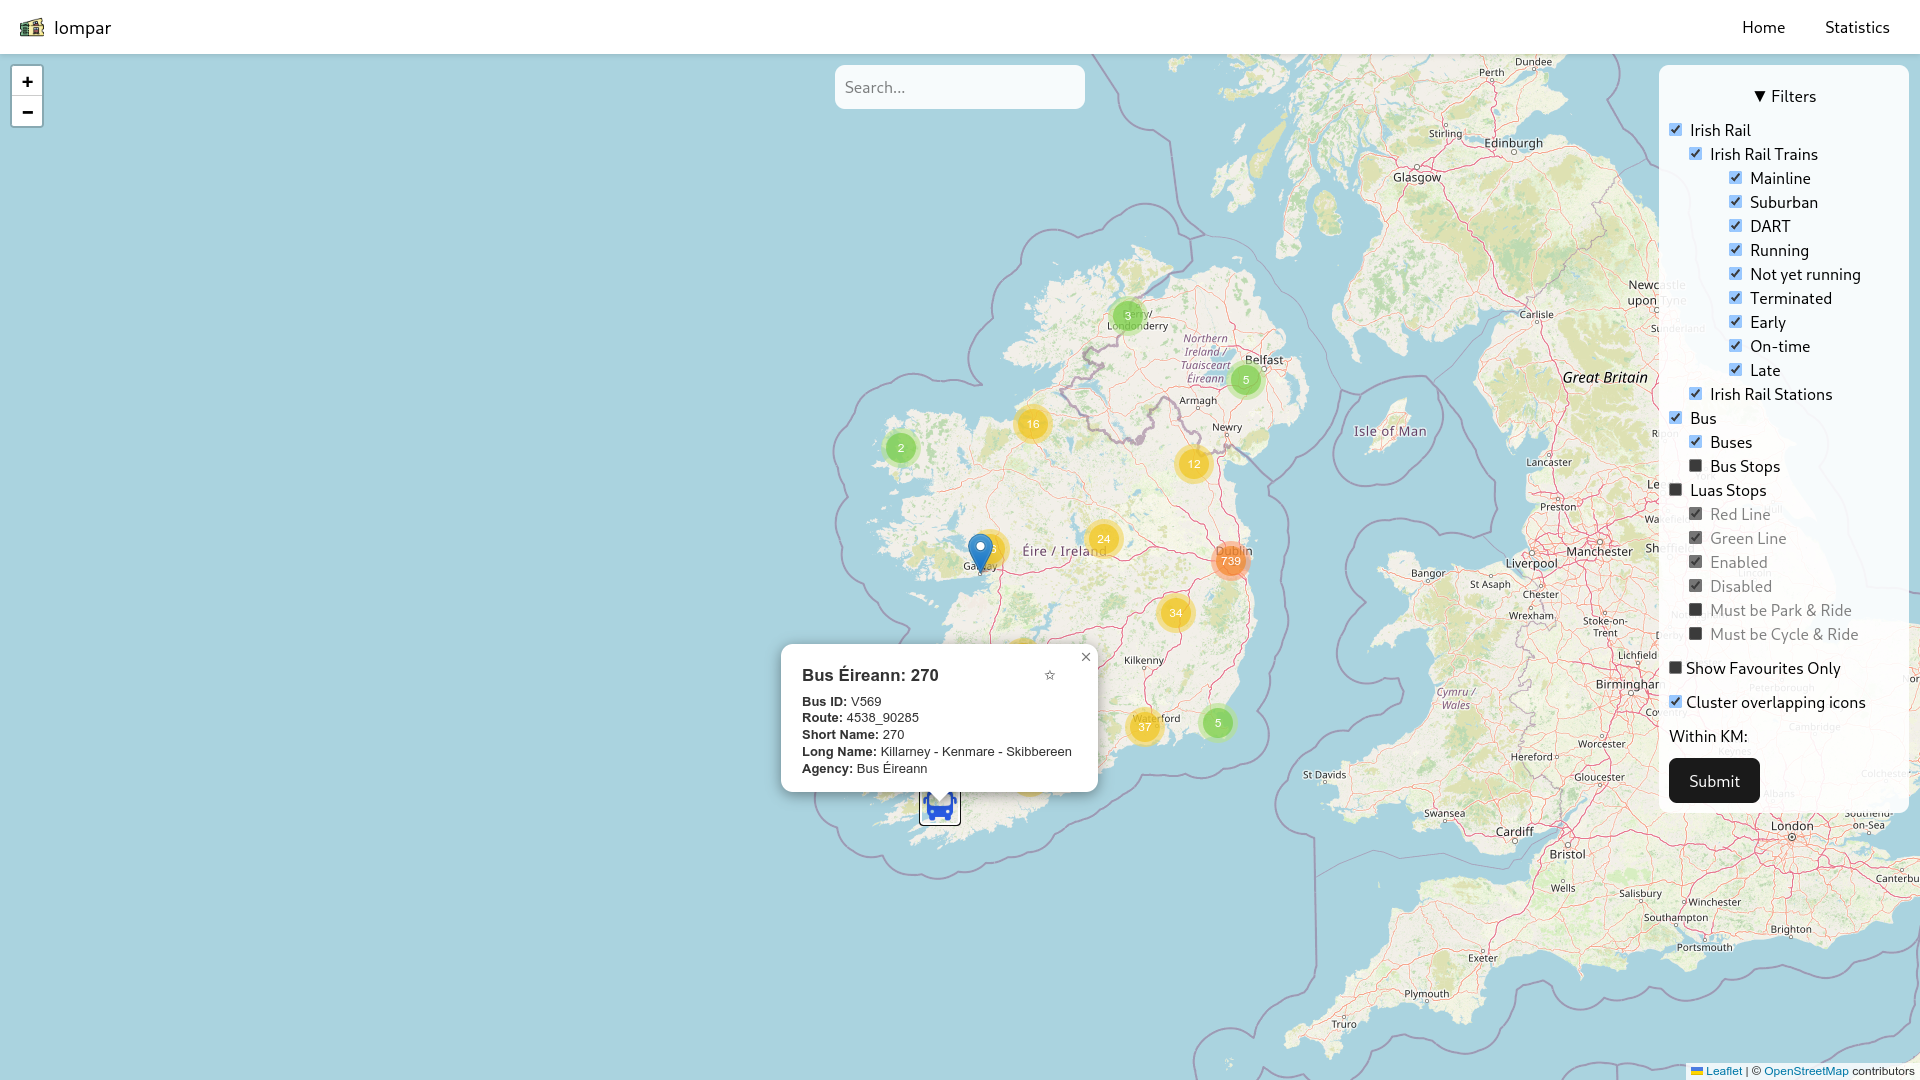
\includegraphics[width=\textwidth]{./images/mainpage.png}
    \caption{Screenshot of the front page of the web application}
\end{figure}

The main page of the application contains a map upon which the live location of each public transport object is marked, a navigation bar, a search bar to filter the vehicles shown on the map, and a filters side-panel which allows the user to select what kind of objects the user wants displayed on the map.
The location markers for each item are clickable, and when clicked, display a pop-up with relevant information about the selected item.
In line with Container/Presentational pattern, the main \verb|App.jsx| file contains the data retrieval \& processing logic, and passes the processed data to presentational components for display. 

\subsubsection{Data Retrieval \& Processing}
The data is retrieved and processed in a function named \mintinline{javascript}{fetchData()}.
When the ``Submit'' button is clicked in the filters side-panel, the function is triggered and sends asynchronous API requests to the \verb|/return_permanent_data| and \verb|/return_transient_data| API endpoints as necessary.
The \verb|App.jsx| file contains a JavaScript object which identifies what checkboxes in the side-panel pertain to \verb|objectType|s in the backend, and which API endpoint they can be sourced from.
When the function is fetching data, it constructs a comma-separated list of selected \verb|objectType|s to send to each API endpoint, thereby making only one request to each API endpoint to avoid unnecessary repeated queries.
\\\\
Originally, the returned data was processed using JavaScript functional array methods\supercite{arraymethods} (very superficially similar to the Java \mintinline{java}{Stream}\supercite{javastream} interface), which allow for the creation of chained operations on arrays, not dissimilar to chained shell operations using the pipe (\mintinline{shell}{|}) operator on UNIX-like systems\supercite{redhatpipe}.
Methods like \mintinline{javascript}{.map()}, \mintinline{javascript}{.reduce()}, etc. are some of the methods covered in JavaScript functional array methods which allow data processing pipelines to be specified in a clean, elegant, \& readable manner.
However, the price of this elegance is slower and less efficient execution:
these array methods add extra layers of abstraction, invoke a new function per element, create intermediate arrays for each result, and (unlike their Java counterparts) do not support short-circuiting and therefore cannot break early.
The modern JavaScript engine also is less efficient at optimising these array methods than simple \mintinline{javascript}{for}-loops.


\printbibliography
\end{document}
